\documentclass[12pt, letterpaper]{article}
%
% File: jtech_memo_template.tex
%
% Written in MS Word by Dr. David Go, Fall 2011 for AME20213
% Translated to LaTex by John Ott
%
% Contact John Ott for any packages you don't have install
% on your latex system.
%
% when printing, "print actual size", "not fit to page"
%
%%%%%%%%% EXACT 1in MARGINS %%%%%%%
%
\setlength\voffset{0pt}%
\setlength\headsep{25pt}% 25pt
\setlength\headheight{12pt}% 12pt
\setlength\topmargin{0pt}%
\addtolength\topmargin{-\headheight}%
\addtolength\topmargin{-\headsep}%

\setlength\hoffset{0pt}
\setlength\marginparwidth{0pt}
\setlength\oddsidemargin{0pt}

\setlength\textwidth{\paperwidth}
\addtolength\textwidth{-2in}
\setlength\textheight{\paperheight}
\addtolength\textheight{-2in}

\setlength{\parindent}{0pt}
\setlength{\textfloatsep}{10pt plus 2pt minus 4pt}

% remove double spacing between bibitem entries
\let\OLDthebibliography\thebibliography
\renewcommand\thebibliography[1]{
  \OLDthebibliography{#1}
  \setlength{\parskip}{0pt}
  \setlength{\itemsep}{0pt plus 0.3ex}
}

\usepackage{graphicx}
\usepackage{subfig}
\usepackage[justification=centering]{caption}
\usepackage{setspace}% for double spacing
\usepackage{mathptmx}% for adobe roman font
\usepackage{amsmath}
\usepackage{tabularx}
\usepackage{booktabs}% to deal with hline spacing issues in tables
\usepackage{hanging}
\usepackage{gensymb}
\usepackage[makeroom]{cancel}
\usepackage{fancyhdr}
\usepackage{enumitem}
\usepackage{hyperref}
\usepackage{xcolor}
\usepackage{mathtools}
\setlength{\headheight}{15.2pt}
%\pagestyle{fancy}
%\rhead{65168}
%\lhead{ }

\newcommand{\tab}{\hspace*{2em}}
\newcommand{\HRule}{\rule{\linewidth}{0.5mm}}
\newcommand{\z}[1]{\text{#1}} % use for times roman font in equations

%%%%%%%%%%%%%%%%%%%%%%%%%%%%%%%%%%%%%%%
\begin{document}
%%%%%%%%%%%%%%%%%%%%%%%%%%%%%%%%%%%%%%%

\makeatletter
\renewcommand\paragraph{% start new line after key
    \@startsection{paragraph}{4}{\z@}%
    {-3.25ex\@plus -1ex \@minus -.2ex}%
    {0.01em}%
    {\normalfont\normalsize\bfseries}}
\makeatother


%%%%%%%%%%%%%%%%%%%%%%%%%%%%%%%%%%%%%%%%%%%%%%%%%%%%%%%
%%%%%%%%%%%%%%%%%%%%%%%%%%%%%%%%%%%%%%%%%%%%%%%%%%%%%%%
%%%%%%%%%%%%%%%%%%%%%%%%%%%%%%%%%%%%%%%%%%%%%%%%%%%%%%%

\begin{center}
{\Large Suggested Changes to followerStopper and smoothUpParams} \\
{Chris Kreienkamp}\\
July 2, 2019
\end{center}

%%%%%%%%%%%%%%%%%%%%%%%%%%%%%%%%%%%%%%%%%%%%%%%%%%%%%%%
%%%%%%%%%%%%%%%%%%%%%%%%%%%%%%%%%%%%%%%%%%%%%%%%%%%%%%%
%%%%%%%%%%%%%%%%%%%%%%%%%%%%%%%%%%%%%%%%%%%%%%%%%%%%%%%

\section{Description}
followerStopper and smoothUpParams are both MATLAB functions used in conjunction in Simulink to control the velocity of an autonomous vehicle. In order to dissipate traffic waves, a vehicle wants to drive at an optimal, or reference, velocity. If the car follows the vehicle directly ahead without following this reference velocity, the car will eventually have to brake hard in order to prevent a crash, and hard braking increases traffic. Sometimes, the car will have to slow down because following the reference velocity would result in a crash. followerStopper is a controller that will tell the car whether it can drive at the reference velocity or if it must drive at some fraction of that velocity. \\
\tab followerStopper takes in the relative velocity between the lead vehicle and autonomous vehicle (AV), the relative distance between the lead vehicle and the autonomous vehicle, and the velocity of the autonomous vehicle to output a command velocity for the AV. followerStopper is a function of r (reference velocity), dx (relative position), dv (relative velocity), v\_AV (autonomous vehicle velocity), dx\_min (minimum distance between lead vehicle and AV), dx\_activate (distance when AV should travel slower than the reference velocity). \\
\tab smoothUpParams edits the reference, or optimal, velocity before it gets to followerStopper in order to prevent harsh and unnecessary acceleration or deceleration. smoothUpParams is a function of the max\_speed (reference velocity), vel (autonomous vehicle velocity), max\_accel (maximum comfortable acceleration for the autonomous vehicle), and max\_decel (maximum comfortable deceleration for the autonomous vehicle. Using these inputs, smoothUpParams edits the reference velocity so that it is a reasonable value when it is sent to the followerStopper controller. Suppose, for example, the speed limit were to change from 10 m/s to 15 m/s and no car was in front of the AV. followerStopper would command the AV to travel at the reference velocity of 15 m/s immediately, but this will result in a large acceleration and an overshoot. smoothUpParams will cause the reference velocity to increase at a slow rate so that followerStopper can still command the reference velocity but it will not result in a large acceleration.

%%%%%%%%%%%%%%%%%%%%%%%%%%%%%%%%%%%%%%%%%%%%%%%%%%%%%%%%
%%%%%%%%%%%%%%%%%%%%%%%%%%%%%%%%%%%%%%%%%%%%%%%%%%%%%%%%
%%%%%%%%%%%%%%%%%%%%%%%%%%%%%%%%%%%%%%%%%%%%%%%%%%%%%%%%

\section{Problem Statement}
A Simulink model was created with two cars. The lead car, initially positioned at 10 m in front of the follower car, was given a synthetic pre-recorded velocity from an actual human driver. The follower car, modeled as an autonomous vehicle, was controlled by smoothUpParams and followerStopper. As seen in Figure 1, there were sharp fluctuations in the reference velocity and the command velocity during the first 5 s, and there were sharp fluctuations in the command velocity around 78 s. Such sharp fluctuations resulted in an unacceptably large acceleration. The goal of this document is to present edits to the MATLAB smoothUpParams and followerStopper codes that will eliminate these sharp fluctuations for this specific lead vehicle velocity profile and for all lead profiles.

\begin{figure}[h!]
\begin{center}
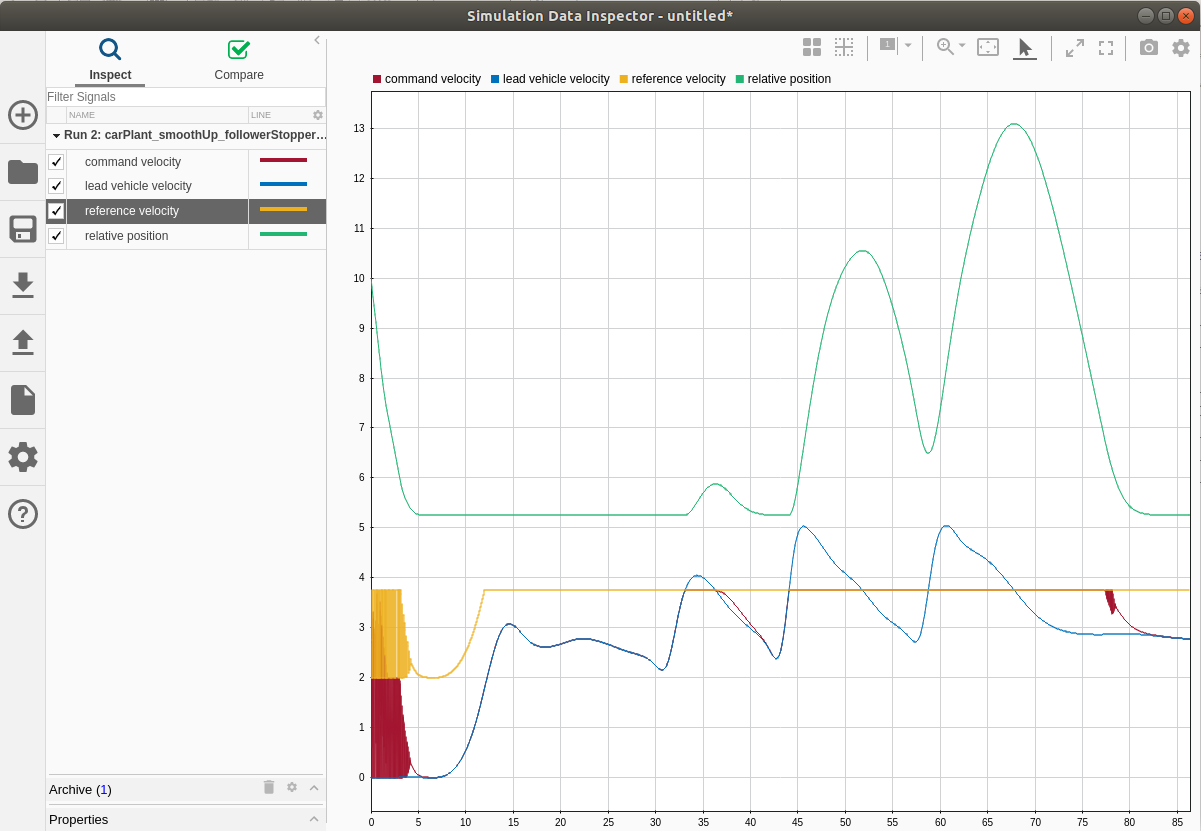
\includegraphics[width=6in]{originalFS_originalSUP_1}
\caption{Original followerStopper and original smoothUpParams.}
\label{default}
\end{center}
\end{figure}

%%%%%%%%%%%%%%%%%%%%%%%%%%%%%%%%%%%%%%%%%%%%%%%%%%%%%%%%
%%%%%%%%%%%%%%%%%%%%%%%%%%%%%%%%%%%%%%%%%%%%%%%%%%%%%%%%
%%%%%%%%%%%%%%%%%%%%%%%%%%%%%%%%%%%%%%%%%%%%%%%%%%%%%%%%

\section{Editing smoothUpParams}
\subsection{Original code}
The original code is displayed on the left side of Figure 2. The function relies on a persistent variable $\mathtt{y}$ to remember what the reference velocity either was or was near, so that if the reference velocity is changed, the code will know it needs to incrementally move toward the new reference velocity. $\mathtt{y}$ can be treated as the output reference velocity from the previous time-step. If there was no previous value of $\mathtt{y}$, it will be set to 0. The code assumes a time-step of 0.05 s, and then proceeds through an $\mathtt{if}$ statement. The $\mathtt{if}$ statement determines if $\mathtt{y}$ is higher than, less than, or within 1 of the $\mathtt{max\_speed}$, which is the reference velocity provided as an input. If $\mathtt{y}$ is higher than the $\mathtt{max\_speed}+1$, then $\mathtt{y}$ will decrease at a deceleration determined by $\mathtt{max\_decel}$. If $\mathtt{y}$ is lower than the $\mathtt{max\_speed}-1$, then $\mathtt{y}$ will decrease at a deceleration determined by $\mathtt{max\_decel}$. Otherwise, $\mathtt{y}$ will be set equal to $\mathtt{max\_speed}$. After exiting the $\mathtt{if}$ statement, the code enters another, checking if $\mathtt{y}$ is less than 1 or 2 and setting it equal to those respective values if so. The rationale is that reference velocity should at least be greater than 0 because followerStopper needs the reference velocity to be a nonzero value in order to give the car a nonzero velocity. If the reference velocity is too fast, followerStopper will protect the AV. The code ends by assuring that $\mathtt{y}$ is at least 1 or 2 and is not less than the current AV velocity by more than 1 m/s.

\begin{figure}
\begin{center}
$\begin{array}{c}
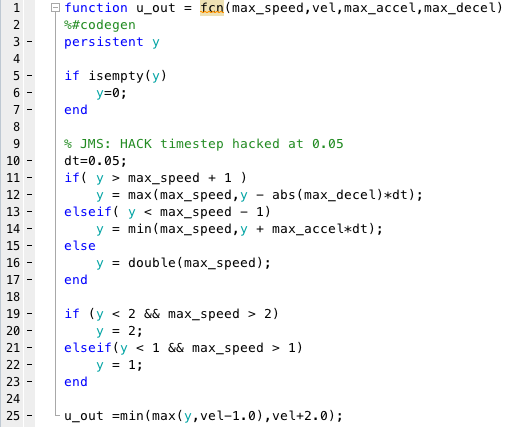
\includegraphics[width=3.0in]{ORIGINAL_smoothUpParams}
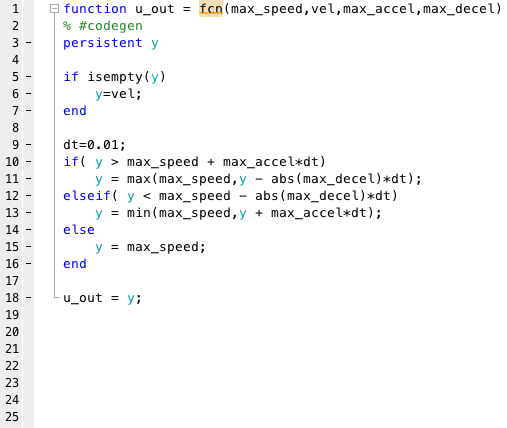
\includegraphics[width=3.0in]{EDITED_smoothUpParams}
\end{array}$
\caption{Original smoothUpParams code (left). Edited smoothUpParams code (right).}
\end{center}
\end{figure}

\subsection{Edited code}
The changes to the original code are described in detail below. Figure 3 displays the new data with the same followerStopper controller but with the edited smoothUpParams controller. As expected, the edits eliminate all sharp oscillations in the reference velocity in yellow. Consequently, the command velocity in red also has less oscillations at the very beginning of the experiment from about 0-1 s.
\subsubsection{Initial value of $\mathtt{y}$}
The edited code is displayed on the right side of Figure 2. Focus will be given to the edits. If there was no previous value of $\mathtt{y}$, it will be set to the current velocity of the autonomous vehicle instead of 0. Consider if the AV is not using followerStopper and then initiates followerStopper when already in motion, perhaps on a ramp to get onto a highway. If there are no cars ahead, followerStopper will tell the AV to follow the reference velocity. If $\mathtt{y}$ is set to the velocity of AV, then a new instantaneous reference velocity will be treated no differently than how the AV would normally react to a new input reference velocity. If $\mathtt{y}=0$, then from line 25 of the original code, the reference velocity $\mathtt{u\_out=vel-1.0}$ until $\mathtt{y>vel-1.0}$, which could take a while if the AV velocity is high because $\mathtt{y}$ can only increment by velocity values that respect the $\mathtt{max\_accel}$ value.
\subsubsection{Time step}
The time-step is changed from $\mathtt{dt=0.05}$ to $\mathtt{dt=0.01}$ because the Simulink model has a time-step of 0.01 s.
\subsubsection{$\mathtt{if}$ statements}
Suppose the AV is traveling at the reference velocity of 5 m/s when it instantaneously changes to 5.9 m/s, but no cars are in front of it. Proceeding through the original code, the code would enter the $\mathtt{else}$ block, then $\mathtt{y=5.9}$. Proceeding to the end, $\mathtt{u\_out=5.9}$. followerStopper would then command 5.9 m/s as the velocity, but this would be clearly wrong as changing from 5.0 m/s to 5.9 m/s over the course of 0.01 s would be an acceleration of 90 $m\over s^2$! Instead, $\mathtt{y} should have entered the \mathtt{elseif}$ block. Assuming $\mathtt{dt=0.01}$ and $\mathtt{max\_accel=1.5}$, then $\mathtt{y=5.15}$, a much more reasonable value. Therefore, the $\mathtt{if}$ statement is changed so that $\mathtt{y}$ will enter the $\mathtt{if}$ block or the $\mathtt{elseif}$ block if it is more than $\mathtt{max\_accel*dt}$ or  $\mathtt{max\_decel*dt}$ away from the  newly input reference velocity $\mathtt{max\_speed}$. \\
\tab In terms of the second  $\mathtt{if}$ statement, it is undesirable to have the reference velocity set to 1 m/s or 2 m/s if the car is not moving. In this particular example, the lead vehicle started 10 m ahead of the AV. followerStopper determined this was a safe distance, so commanded the AV to travel at the reference velocity. Therefore, the AV had to go from 0 m/s to 2 m/s over the course of 0.01 s, resulting in an acceleration of 200$m\over s^2$!
\subsubsection{$\mathtt{u\_out}$}
As described above, it is undesirable to use any reference velocity other than one that is spaced away from the previous reference velocity by an acceleration multiplied by a time-step. $\mathtt{y}$ was already computed to serve as this value, so it can be directly used for the new reference velocity $\mathtt{u\_out}$.

\begin{figure}[h!]
\begin{center}
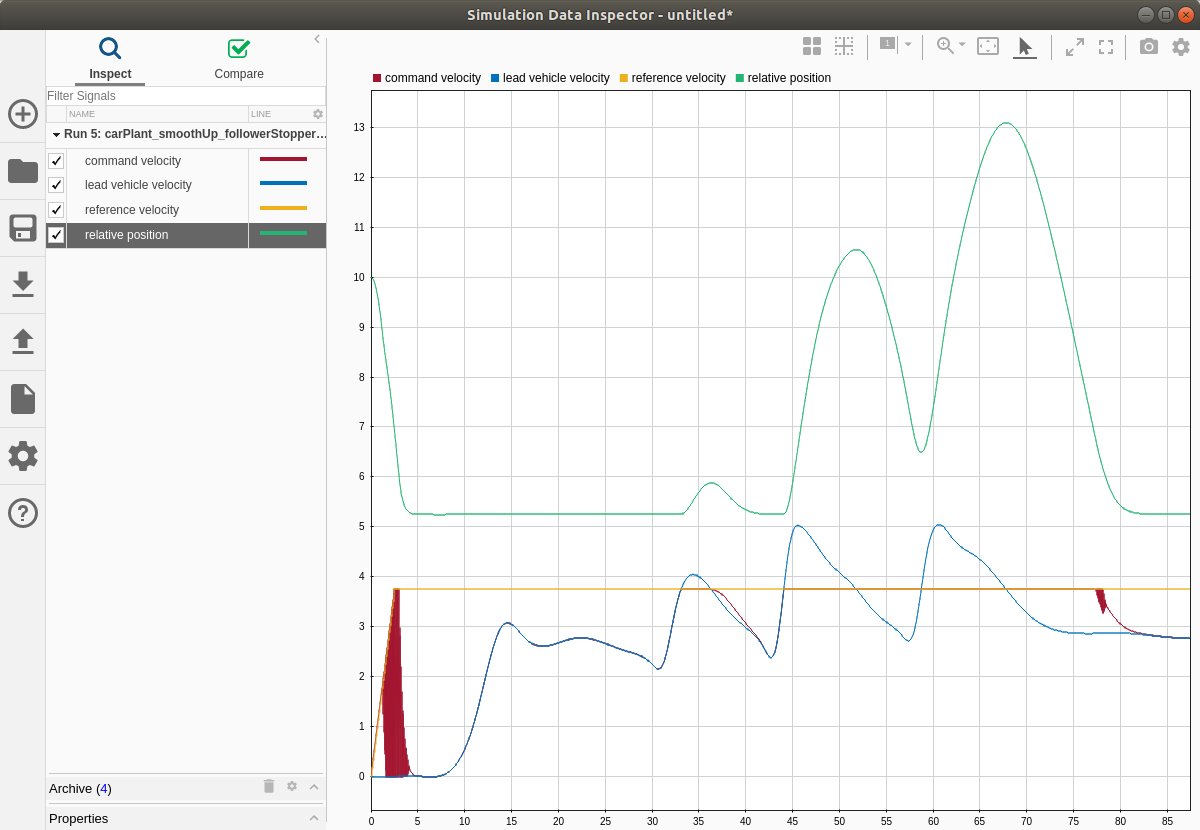
\includegraphics[width=6in]{originalFS_editedSUP_1}
\caption{Original followerStopper and edited smoothUpParams.}
\label{default}
\end{center}
\end{figure}

%%%%%%%%%%%%%%%%%%%%%%%%%%%%%%%%%%%%%%%%%%%%%%%%%%%%%%%%
%%%%%%%%%%%%%%%%%%%%%%%%%%%%%%%%%%%%%%%%%%%%%%%%%%%%%%%%
%%%%%%%%%%%%%%%%%%%%%%%%%%%%%%%%%%%%%%%%%%%%%%%%%%%%%%%%

\section{Editing followerStopper}
The changes to the original code are described in detail below. Figure 5 displays the new data with the edited (part 1) followerStopper controller and with the edited smoothUpParams controller. Though the reference velocity remains smooth, the commanded velocity in red is only slightly improved. As seen in the first few seconds, comparing the plot in Figure 5 to the previous plot in Figure 3 reveals that the oscillations at the very beginning are less dense, yet they occur for a longer time period. The oscillations at around 78 s did not change.  Figure 7 displays the new data with the edited (part 2) followerStopper controller and with the edited smoothUpParams controller. In this figure, the acceleration of the AV is also added in light green to show that the acceleration never goes above 1.5 $m\over s^2$. There are still small oscillations, but they are dramatically reduced from previous versions of smoothUpParams and followerStopper and are acceptable.
\subsection{Original code}
The original code is displayed on the left side of Figure 4, and the edited (part 1) code is on the right. The code, except for the last $\mathtt{if}$ statement, exactly follows the equations for FollowerStopper as laid out in "Real-Time Distance Estimation and Filtering of Vehicle Headways for Smoothing of Traffic Waves." That is,
\begin{eqnarray}
x 			&=& x_{lead}-x_{AV}-L \\
\dot x 		&=& v_{lead}-v_{AV} \\
\xi_j(\dot x)	&=& \omega_j + {1\over 2\alpha_j}(\dot x^*)^2 \ \ {\rm for \ \ j=1, 2, 3} \\
u &=& \begin{dcases}
        0 			& x\leq \xi_1 \\
        v{x-\xi_1\over\xi_2-\xi_1} 	& \xi_1\le x\leq \xi_2 \\
        v+(r-v){x-\xi_2\over\xi_3-\xi_2}			& \xi_2\le x\leq \xi_3 \\
        r 			& \xi_3\le x \\
    \end{dcases}
\end{eqnarray}
where $\dot x^* = min(\dot x, 0)$. $r$ is the reference velocity as taken from the output of smoothUpParams, $u$ is the command velocity that is sent to the AV, and $\alpha_j$ and $\omega_j$ are parameters.

\begin{figure} [h]
\begin{center}
$\begin{array}{c}
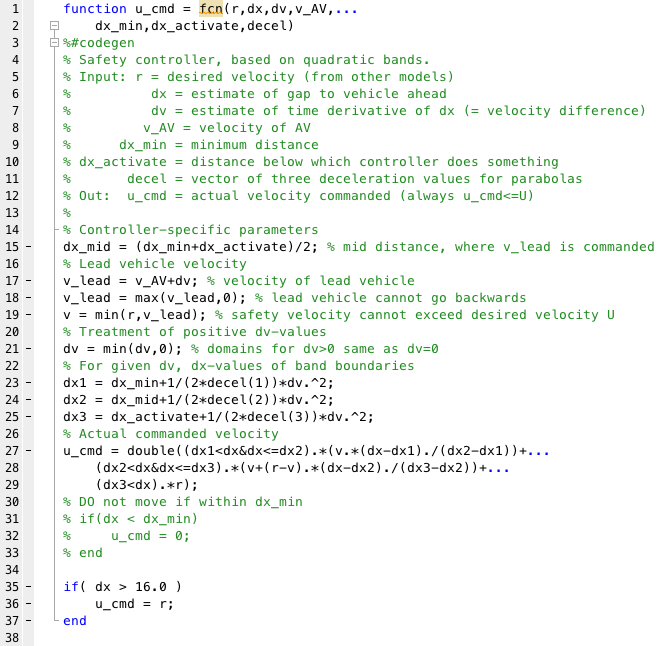
\includegraphics[width=3.0in]{ORIGINAL_followerStopper}
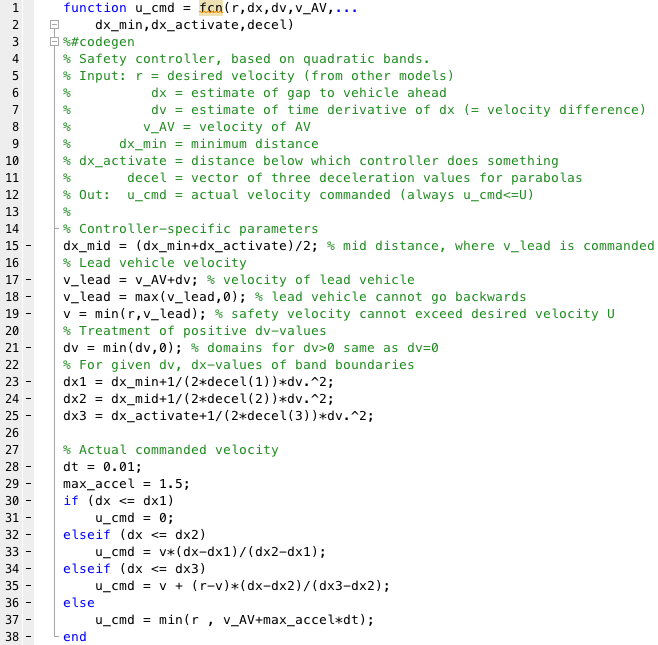
\includegraphics[width=3.0in]{EDITED_followerStopper}
\end{array}$
\caption{Original followerStopper code (left). Edited (part 1) followerStopper code (right).}
\end{center}
\end{figure}

\subsection{Edited code part 1}
\subsubsection{$\mathtt{if}$ statement}
The original code is easy to follow until line 27. In that line, the original code does not account for the possibility $\mathtt{dx<=dx1}$. A similar concept is employed on line 32, but it is commented out and it is not entirely accurate because it compares $\mathtt{dx}$ to $\mathtt{dx\_min}$, not $\mathtt{dx1}$ as outlined in equation 4. Additionally, in line 35, the value $\mathtt{16.0}$ seems to be arbitrarily chosen when in reality $\mathtt{u\_cmd}$ should equal the reference velocity only when $\mathtt{dx3<dx}$. The $\mathtt{if}$ statement follows equation 4 exactly. The only variation is line 37 in the edited code (part 1) in Figure 4 when $\mathtt{u\_cmd=min(r , v\_AV+max\_accel*dt)}$ because the car should not accelerate faster than its maximum desired acceleration to get to the reference velocity.

\begin{figure}[h!]
\begin{center}
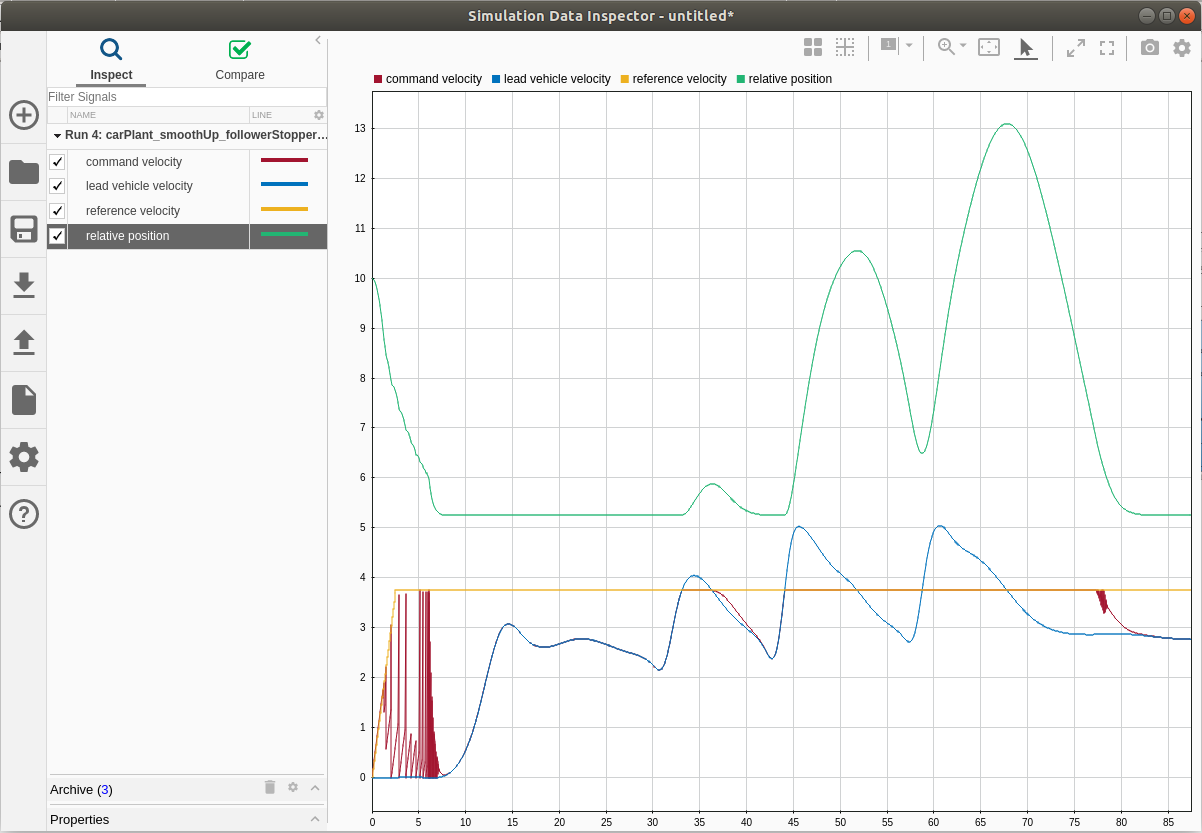
\includegraphics[width=6in]{editedFS_editedSUP_1}
\caption{Edited (part 1) followerStopper and edited smoothUpParams.}
\label{default}
\end{center}
\end{figure}

\subsection{Edited code part 2}
Figure 6 displays the edited (part 2) and (part 3) code. They do the same thing, except (part 3) uses a piecewise setup for $\tt{u\_cmd}$ rather than the $\tt{if}$ statement.
\subsubsection{$\mathtt{smoothChange}$}
After spending some time looking at the oscillations, it was revealed that the sharp jumps occur when the relative distance $\mathtt{dx}$ crosses into a different piecewise area of the FollowerStopper in equation 4. If it was traveling at the reference velocity, the followerStopper edited code (part 1) made sure that it did not immediately travel at the reference velocity, but would incrementally work up to it. At points the AV would cross the $\mathtt{dx3}$ barrier, shooting up because that piecewise section calculated the command velocity $\mathtt{u}$ to be a large fraction of the much higher reference velocity. To solve this problem, a $\mathtt{smoothChange}$ variable, designed on line 30 in Figure 6, assured that no matter in what piecewise area that FollowerStopper was operating, it would not accelerate faster than the maximum acceleration. Though this could be tuned to deceleration as well, it is not desirable because FollowerStopper should not be limited in how quickly it can decelerate in case it needs to brake at full force to prevent a crash. Acceleration, however, is entirely dependent on rider comfort.

\begin{figure}[h]
\begin{center}
$\begin{array}{c}
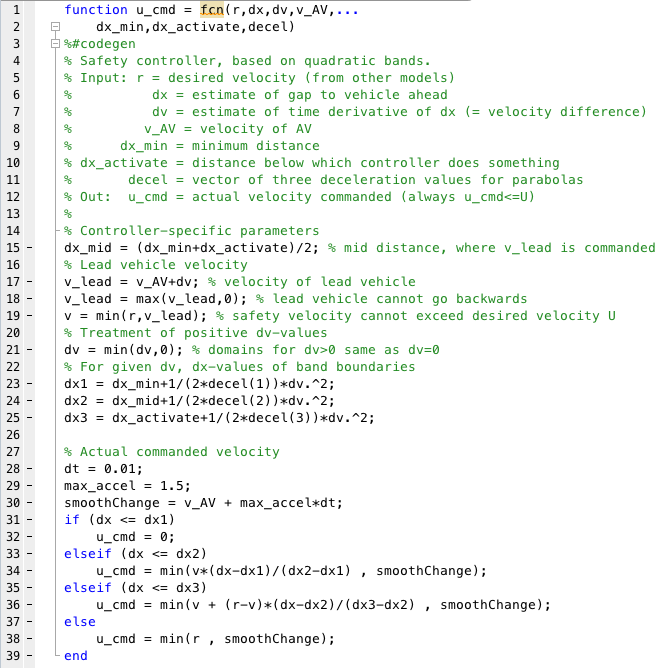
\includegraphics[width=3in]{EDITED2_followerStopper}
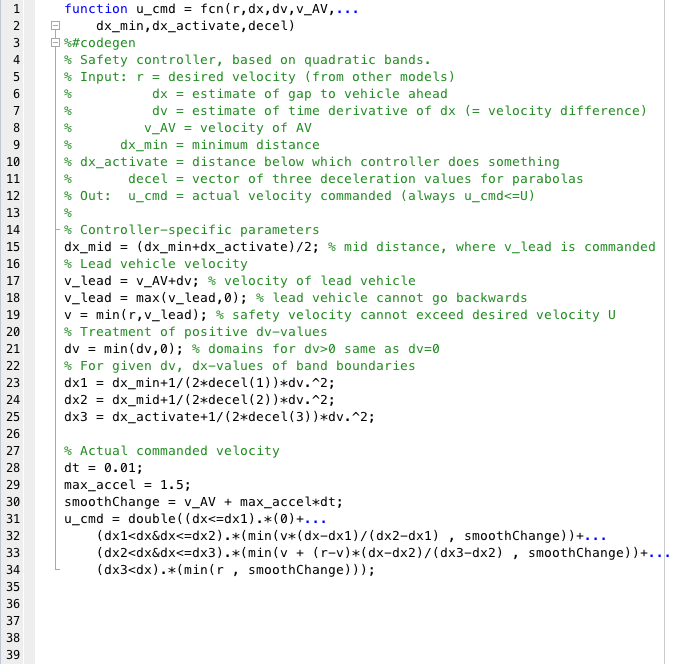
\includegraphics[width=3in]{EDITED3_followerStopper}
\end{array}$
\caption{Edited (part 2) followerStopper code and edited (part 3) of followerStopper code.}
\label{default}
\end{center}
\end{figure}

\begin{figure}[h!]
\begin{center}
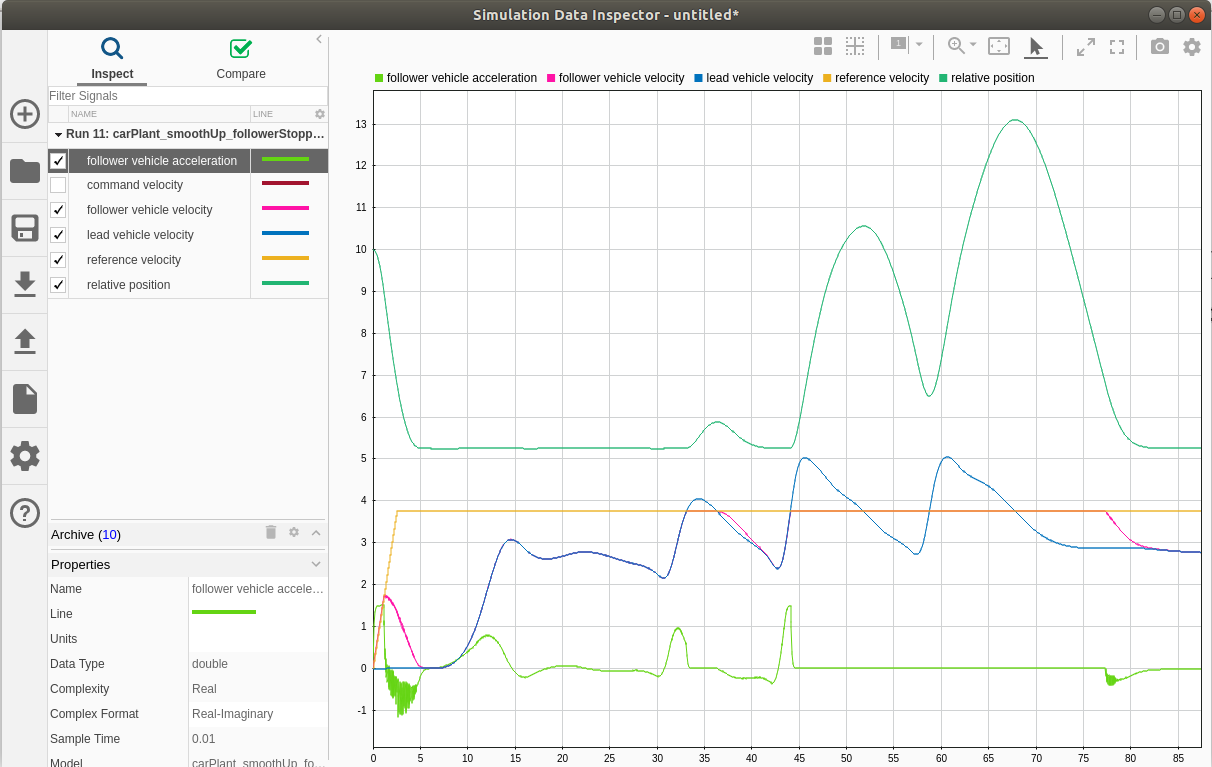
\includegraphics[width=6in]{edited2FS_editedSUP_1}
\caption{Edited (part 2) followerStopper and edited smoothUpParams.}
\label{default}
\end{center}
\end{figure}

%%%%%%%%%%%%%%%%%%%%%%%%%%%%%%%%%%%%%%%%%%%%%%%%%%%%%%%%
%%%%%%%%%%%%%%%%%%%%%%%%%%%%%%%%%%%%%%%%%%%%%%%%%%%%%%%%
%%%%%%%%%%%%%%%%%%%%%%%%%%%%%%%%%%%%%%%%%%%%%%%%%%%%%%%%

\section{Appendix}
Below are more figures for reference.

\begin{figure}[h]
\begin{center}
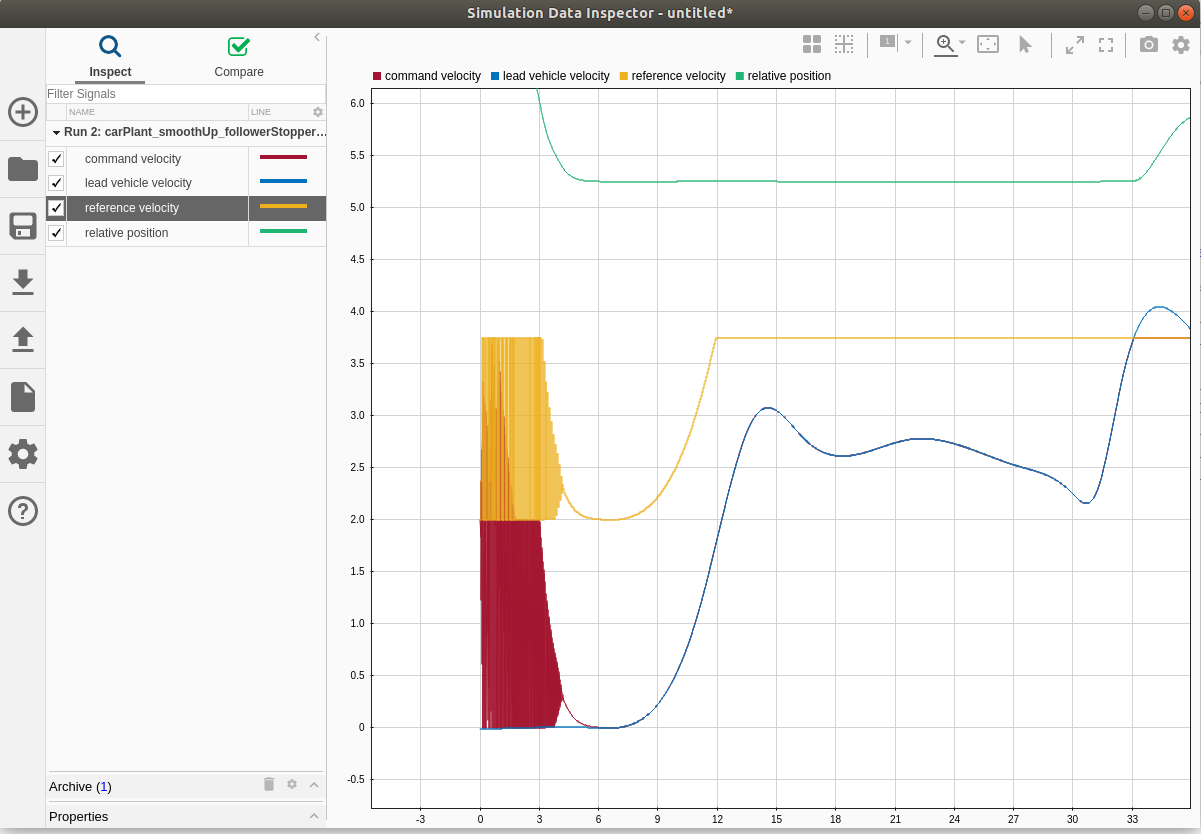
\includegraphics[width=4in]{originalFS_originalSUP_2}
\caption{Original followerStopper and original smoothUpParams at the first oscillation set.}
\label{default}
\end{center}
\end{figure}

\begin{figure}[h]
\begin{center}
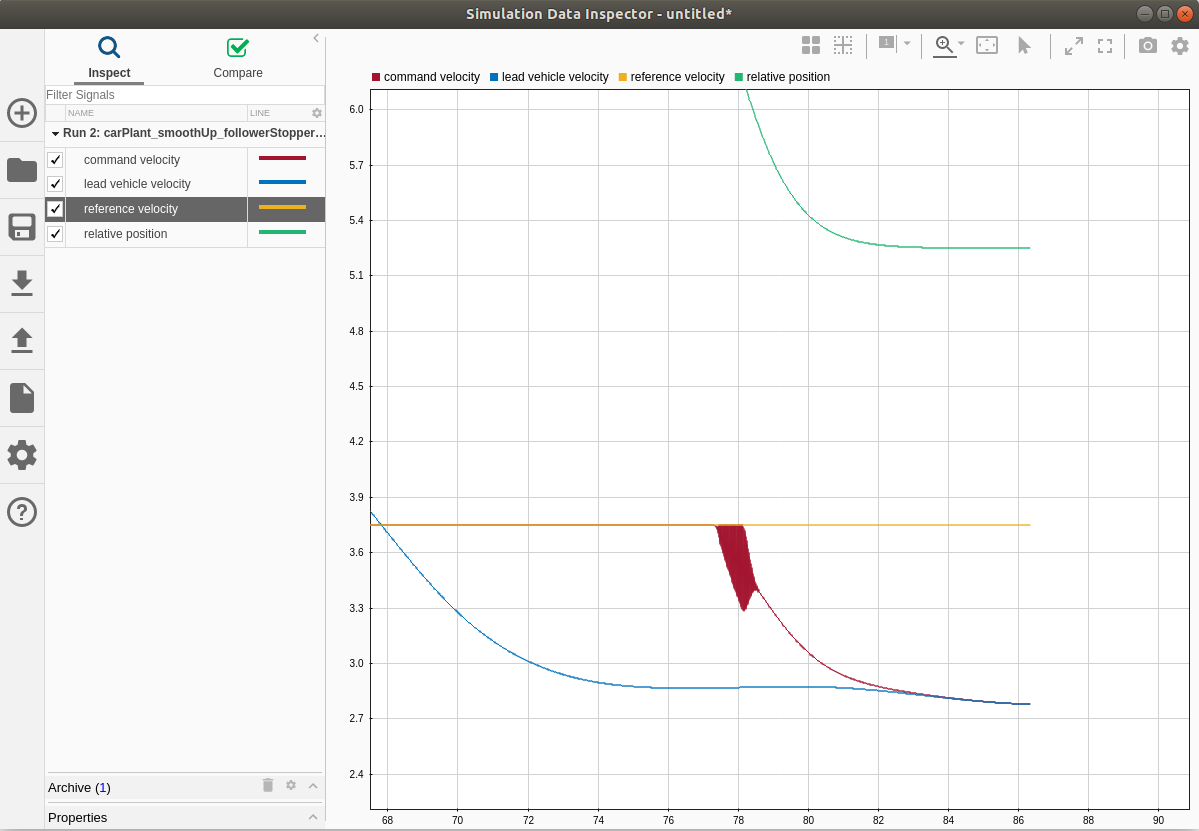
\includegraphics[width=4in]{originalFS_originalSUP_3}
\caption{Original followerStopper and original smoothUpParams at the second oscillation set.}
\label{default}
\end{center}

\end{figure}
\begin{figure}[h]
\begin{center}
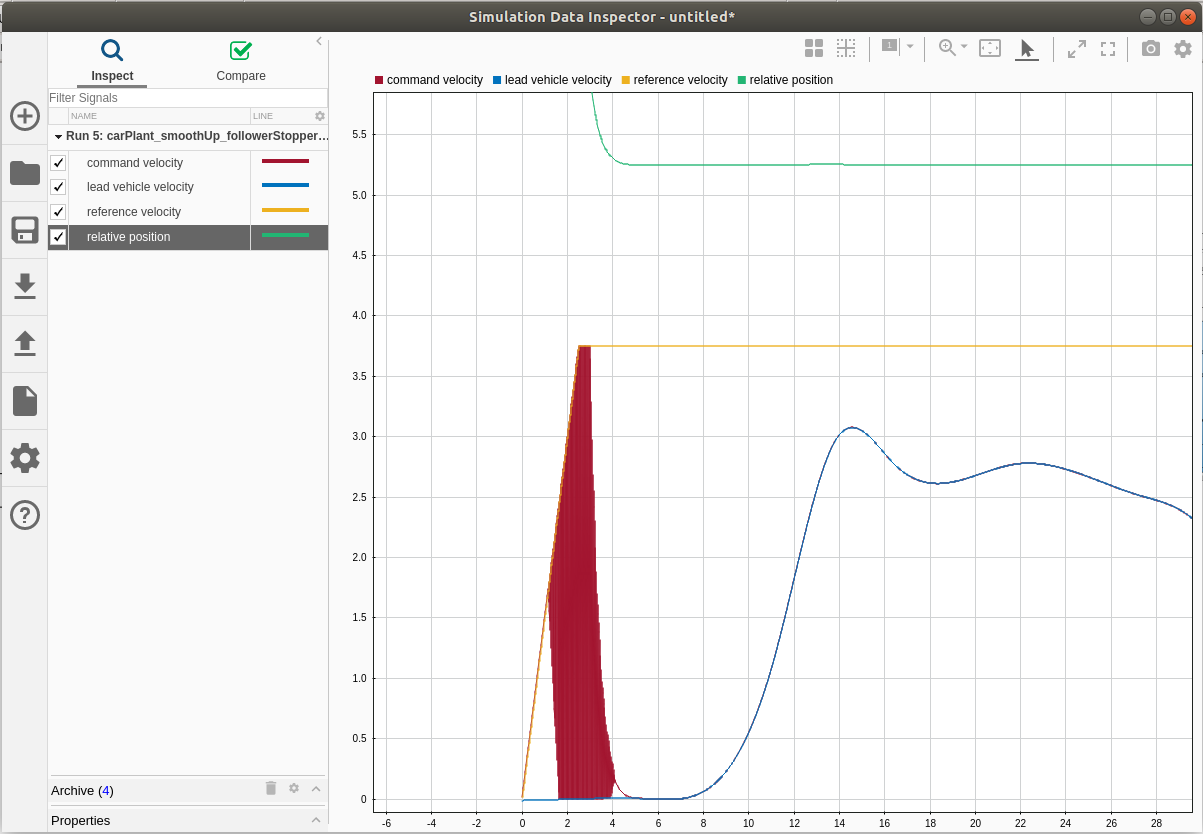
\includegraphics[width=4in]{originalFS_editedSUP_2}
\caption{Original followerStopper and edited smoothUpParams at the first oscillation set.}
\label{default}
\end{center}
\end{figure}

\begin{figure}[h]
\begin{center}
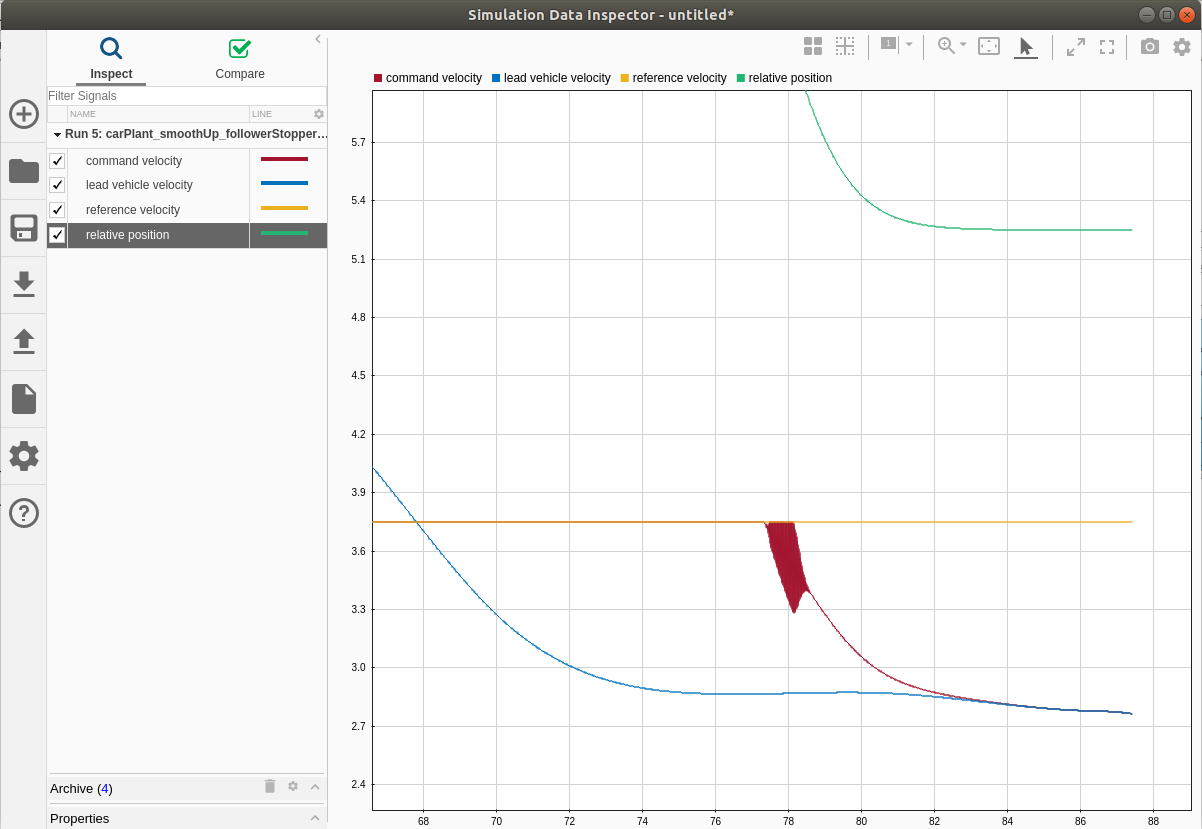
\includegraphics[width=4in]{originalFS_editedSUP_3}
\caption{Original followerStopper and edited smoothUpParams at the second oscillation set.}
\label{default}
\end{center}
\end{figure}

\begin{figure}[h]
\begin{center}
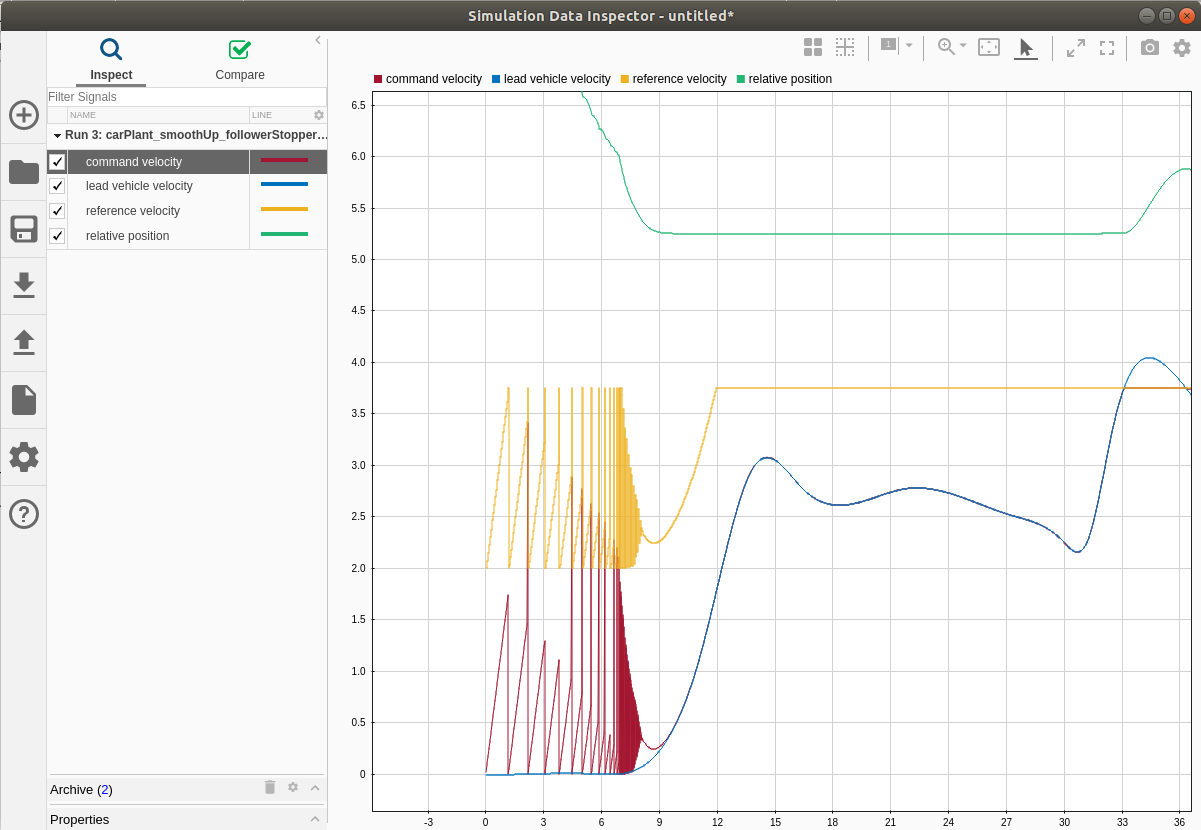
\includegraphics[width=4in]{editedFS_originalSUP_2}
\caption{Edited (part 1) followerStopper and original smoothUpParams at the first oscillation set.}
\label{default}
\end{center}
\end{figure}

\begin{figure}[h]
\begin{center}
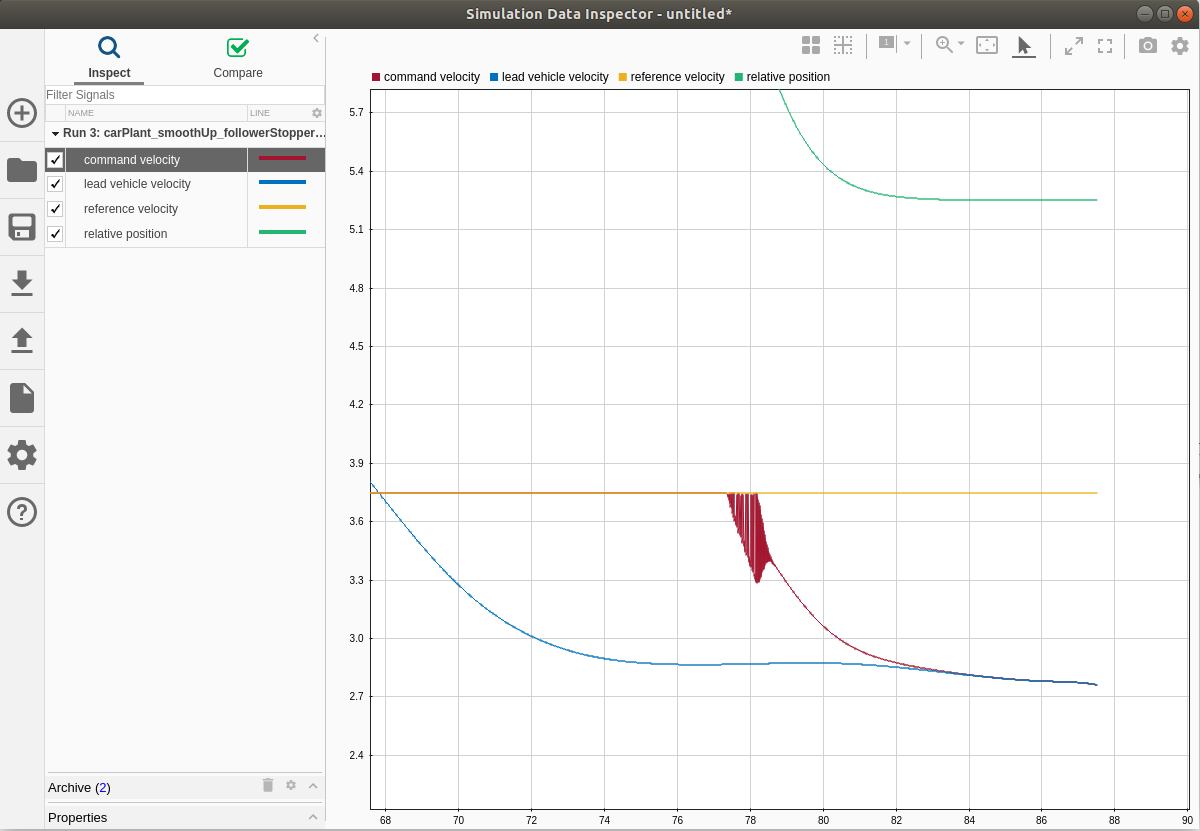
\includegraphics[width=4in]{editedFS_originalSUP_3}
\caption{Edited (part 1) followerStopper and original smoothUpParams at the second oscillation set.}
\label{default}
\end{center}
\end{figure}

\begin{figure}[h]
\begin{center}
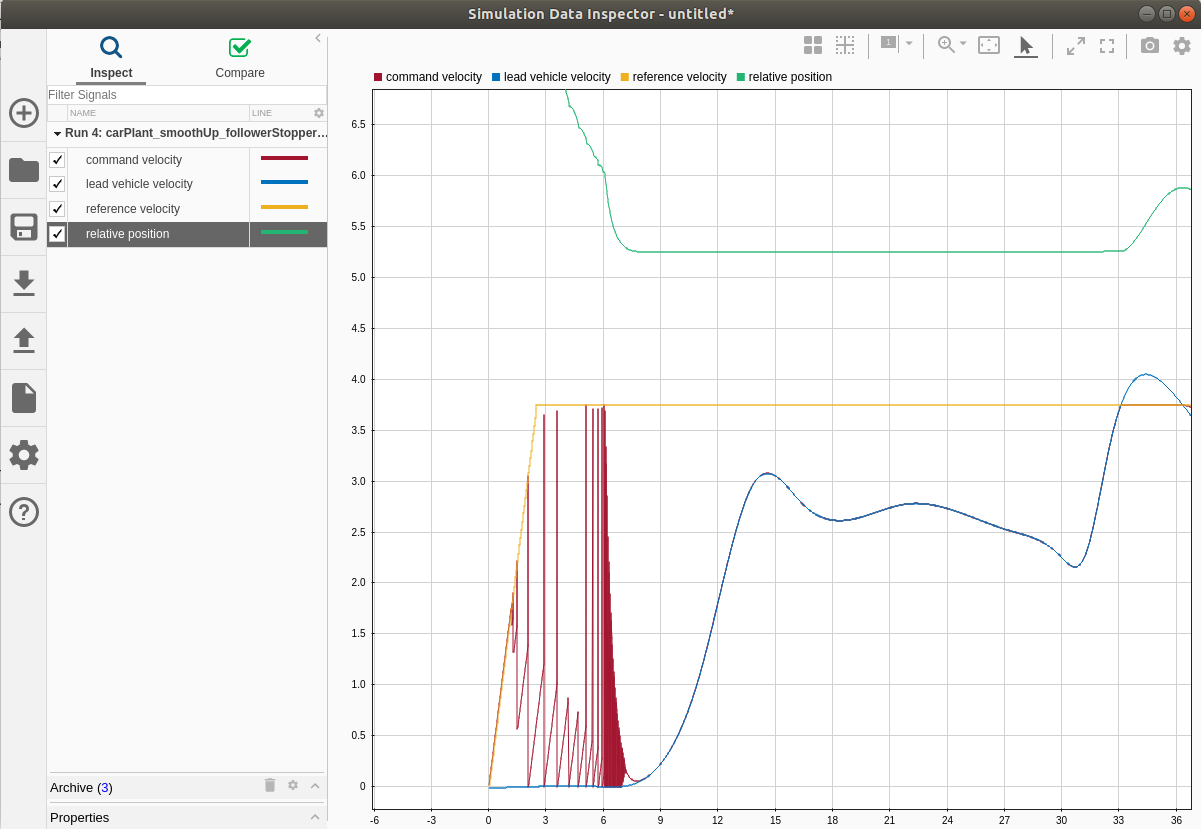
\includegraphics[width=4in]{editedFS_editedSUP_2}
\caption{Edited (part 1) followerStopper and edited smoothUpParams at the first oscillation set.}
\label{default}
\end{center}
\end{figure}

\begin{figure}[h]
\begin{center}
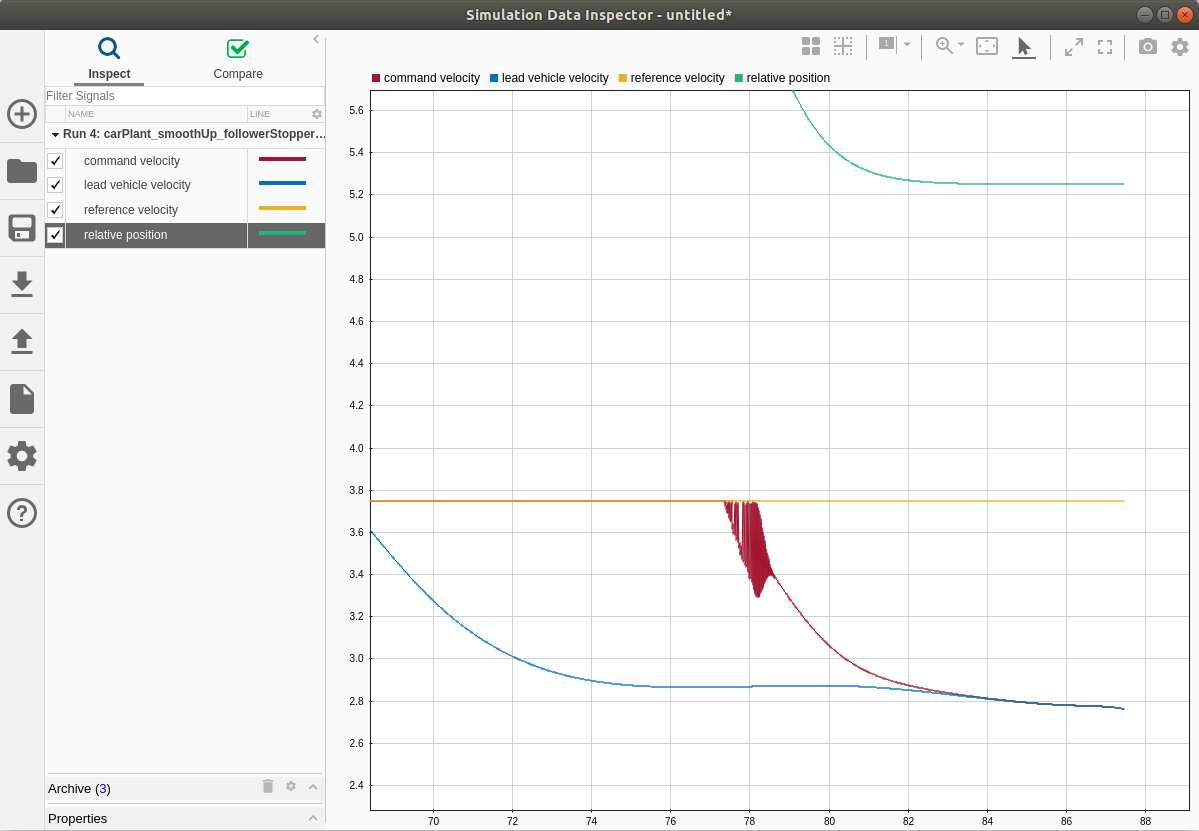
\includegraphics[width=4in]{editedFS_editedSUP_3}
\caption{Edited (part 1) followerStopper and edited smoothUpParams at the second oscillation set.}
\label{default}
\end{center}
\end{figure}

\begin{figure}[h]
\begin{center}
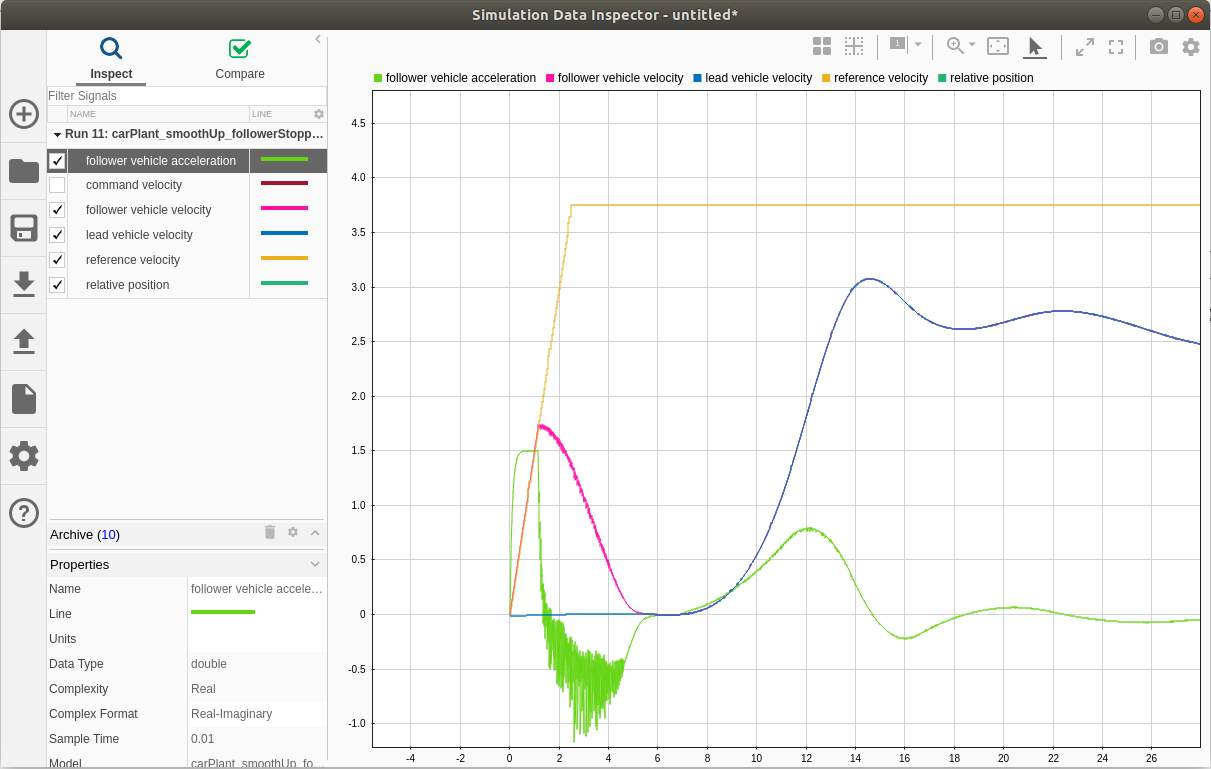
\includegraphics[width=4in]{edited2FS_editedSUP_2}
\caption{Edited (part 2) followerStopper and edited smoothUpParams at the first oscillation set.}
\label{default}
\end{center}
\end{figure}

\begin{figure}[h]
\begin{center}
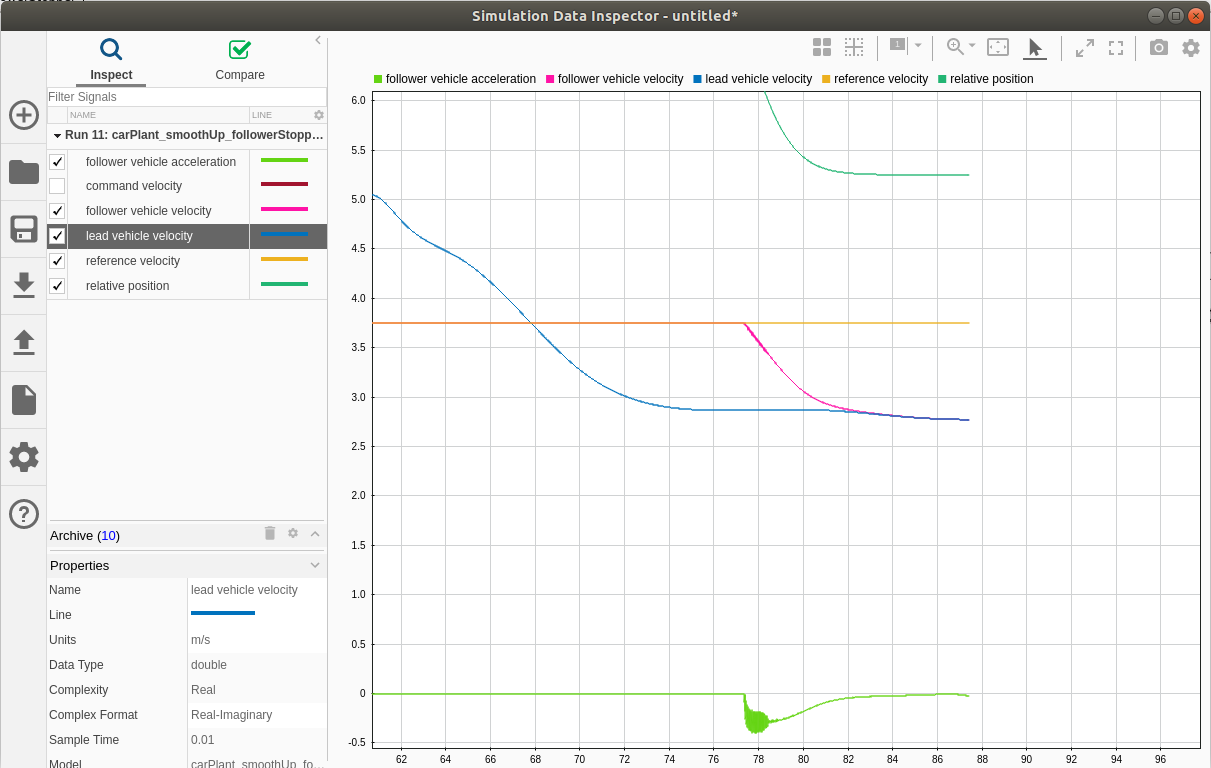
\includegraphics[width=4in]{edited2FS_editedSUP_3}
\caption{Edited (part 2) followerStopper and edited smoothUpParams at the second oscillation set.}
\label{default}
\end{center}
\end{figure}

\end{document}